\frontmatter												%Seitennumerierung
\pagenumbering{Roman}										%Römische Zahlen
\addtocounter{page}{2}

\newcommand{\doublesignature}[2]{%
  \parbox{\textwidth}{
    \hfill
    \parbox{7cm}{
      \centering
      \rule{6cm}{1pt}\\
      #1
    }
    \parbox{7cm}{
      \centering
      \rule{6cm}{1pt}\\
      #2
    }
  }
  \mbox{}\\
  \mbox{}\\
  \mbox{}\\
  \mbox{}\\
}
\newcommand{\singlesignature}[2]{%
  \parbox{\textwidth}{
    \hfill
    \parbox{7cm}{
      \centering
      \rule{6cm}{1pt}\\
      #1
    }
  }
  \mbox{}\\
  \mbox{}\\
  \mbox{}\\
  \mbox{}\\
}

\vspace*{20pt}

\section*{Eidesstattliche Erklärung}
\label{sec:eidesstattliche-erklaerung}
Ich erkläre an Eides statt, dass ich die vorliegende Arbeit selbstständig verfasst, andere als die angegebenen
Quellen/Hilfsmittel nicht benutzt und die den benutzten Quellen wörtlich und inhaltlich entnommenen
Stellen als solche kenntlich gemacht habe.\\
\\
Arnfels, am 18. März 2018\\

\vskip 1cm

\doublesignature{Stefan Hörmann}{Nicolas Perl}
\singlesignature{Alois Vollmaier}

\vskip 5cm

\clearpage

\newpage
\thispagestyle{empty}
\mbox{}

\clearpage

\section*{Danksagung}
\label{sec:danksagung}
An dieser Stelle möchten wir, Stefan Hörmann, Nicolas Perl und Alois Vollmaier, uns im Rahmen der Diplomarbeit bei allen bedanken, die uns unterstützt und betreut haben.
Im Speziellen sind dies einerseits unsere Betreuer, Dipl.-Ing Dr. Gerhand Pretterhofer und Dipl.-Ing Manfred Steiner.
Mithilfe deren fundamental wichtigen Ideen und deren Fachwissen ist es uns gelungen, dieses Werk zu kreieren.
Des Weiteren möchten wir uns herzlich bei Herrn Ing. Konrad Wilhelm und bei Herrn Ing. Dipl.-Päd. St.-Rat Reinhard Semlitsch bedanken, welche uns beim Fertigungsprozess enorm unterstützten und eine elementare Rolle spielten.
Nicht zuletzt gebührt ein ganz spezieller Dank unseren Familien, Verwandten und Freunden, welche und in dieser einschneidenten Zeit voll und ganz unterstützten.
\clearpage

\newpage
\thispagestyle{empty}
\mbox{}

\clearpage

\section*{Abstract}
\label{sec:abstract}
"Lorem ipsum dolor sit amet, consectetur adipiscing elit, sed do eiusmod tempor incididunt ut labore et dolore magna aliqua. Ut enim ad minim veniam, quis nostrud exercitation ullamco laboris nisi ut aliquip ex ea commodo consequat. Duis aute irure dolor in reprehenderit in voluptate velit esse cillum dolore eu fugiat nulla pariatur. Excepteur sint occaecat cupidatat non proident, sunt in culpa qui officia deserunt mollit anim id est laborum."
"Sed ut perspiciatis unde omnis iste natus error sit voluptatem accusantium doloremque laudantium, totam rem aperiam, eaque ipsa quae ab illo inventore veritatis et quasi architecto beatae vitae dicta sunt explicabo. Nemo enim ipsam voluptatem quia voluptas sit aspernatur aut odit aut fugit, sed quia consequuntur magni dolores eos qui ratione voluptatem sequi nesciunt. Neque porro quisquam est, qui dolorem ipsum quia dolor sit amet, consectetur, adipisci velit, sed quia non numquam eius modi tempora incidunt ut labore et dolore magnam aliquam quaerat voluptatem. Ut enim ad minima veniam, quis nostrum exercitationem ullam corporis suscipit laboriosam, nisi ut aliquid ex ea commodi consequatur? Quis autem vel eum iure reprehenderit qui in ea voluptate velit esse quam nihil molestiae consequatur, vel illum qui dolorem eum fugiat quo voluptas nulla pariatur?"

\section*{Zusammenfassung}
"Lorem ipsum dolor sit amet, consectetur adipiscing elit, sed do eiusmod tempor incididunt ut labore et dolore magna aliqua. Ut enim ad minim veniam, quis nostrud exercitation ullamco laboris nisi ut aliquip ex ea commodo consequat. Duis aute irure dolor in reprehenderit in voluptate velit esse cillum dolore eu fugiat nulla pariatur. Excepteur sint occaecat cupidatat non proident, sunt in culpa qui officia deserunt mollit anim id est laborum."
"Sed ut perspiciatis unde omnis iste natus error sit voluptatem accusantium doloremque laudantium, totam rem aperiam, eaque ipsa quae ab illo inventore veritatis et quasi architecto beatae vitae dicta sunt explicabo. Nemo enim ipsam voluptatem quia voluptas sit aspernatur aut odit aut fugit, sed quia consequuntur magni dolores eos qui ratione voluptatem sequi nesciunt. Neque porro quisquam est, qui dolorem ipsum quia dolor sit amet, consectetur, adipisci velit, sed quia non numquam eius modi tempora incidunt ut labore et dolore magnam aliquam quaerat voluptatem. Ut enim ad minima veniam, quis nostrum exercitationem ullam corporis suscipit laboriosam, nisi ut aliquid ex ea commodi consequatur? Quis autem vel eum iure reprehenderit qui in ea voluptate velit esse quam nihil molestiae consequatur, vel illum qui dolorem eum fugiat quo voluptas nulla pariatur?"
\clearpage

\newpage
\thispagestyle{empty}
\mbox{}

\clearpage

\subsection*{Gender Erklärung}
\label{sec:gender-erklaerung}
Aus Gründen der besseren Lesbarkeit wird in dieser Arbeit die Sprachform des generischen Maskulinums angewendet. Es wird an dieser Stelle darauf hingewiesen, dass die ausschließliche Verwendung der männlichen Form geschlechtsunabhängig verstanden werden soll.

\subsection*{Über dieses Dokument}
\label{sec:ueber-dokument}
Diese Arbeit wurde in \LaTeX{} verfasst. Diese Art der Dokumentation bietet gegenüber den normalen Textverarbeitungen gewisse Vorteile hinsichtlich der Formatierung und des Einbindens von Grafiken. Auch Formeln können sehr einfach und effizient angegegeben werden. Die Rohfassung des Dokuments befindet sich auf dem Arnfelser Gitweb Server der HTBLA Kaindorf Abteilung Mechatronik.

\clearpage

\newpage
\thispagestyle{empty}
\mbox{}

\clearpage

\section*{Projektteam}
\label{sec:projektteam}

\subsection*{Stefan Hörmann}
\begin{wrapfigure}[10]{0}{0.5\textwidth}
\begin{center}
  \vspace{-20mm}
  
\includegraphics[width=0.3\textwidth]{fig/H.jpg}
\end{center}
\end{wrapfigure}
\mbox{}\\
\mbox{}\\
\textbf{Aufgabenbereich}:\\
Mechanik\\
\textbf{Betreuer}:\\
Dr. Dipl-Ing. Gerhard Pretterhofer
\mbox{}\\
\mbox{}\\
\mbox{}\\
\subsection*{Nicolas Perl}
\begin{wrapfigure}[10]{0}{0.5\textwidth}
\begin{center}
  \vspace{-20mm}
  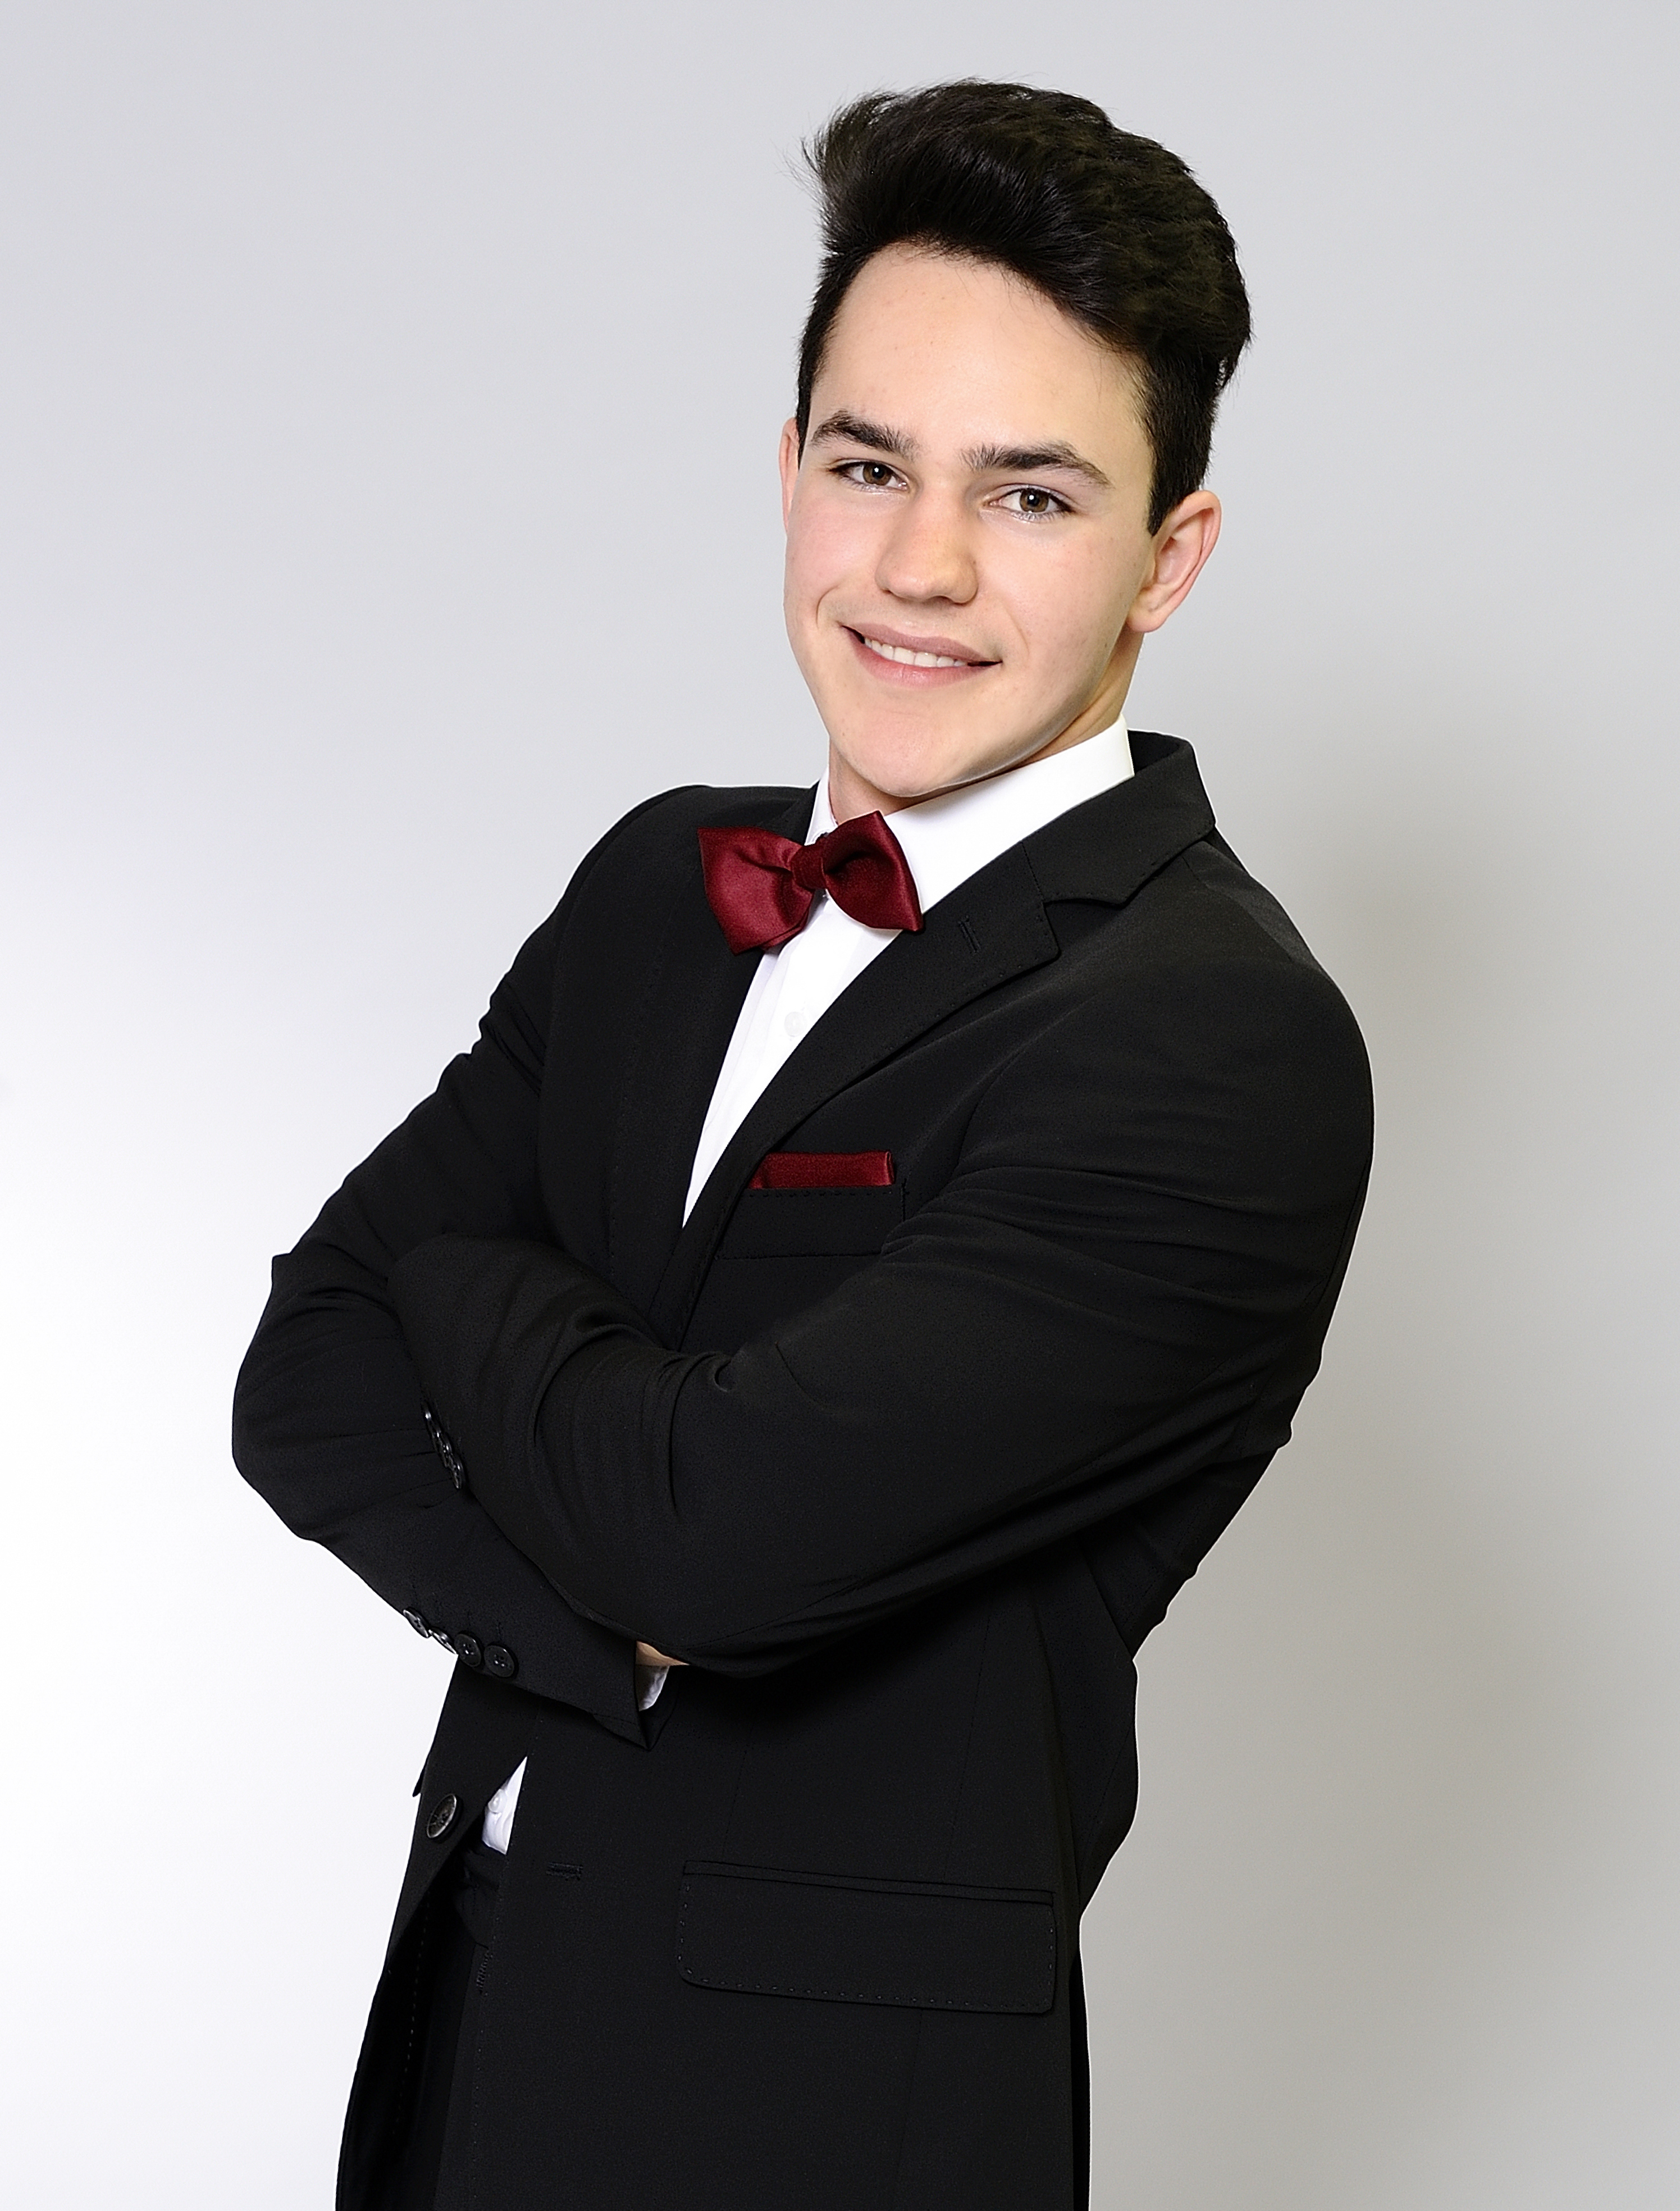
\includegraphics[width=0.3\textwidth]{fig/P.jpg}
\end{center}
\end{wrapfigure}
\mbox{}\\
\mbox{}\\
\textbf{Aufgabenbereich}:\\
Elektronik\\
\textbf{Betreuer}:\\
Dipl-Ing. Manfred Steiner
\mbox{}\\
\mbox{}\\
\mbox{}\\
\subsection*{Alois Vollmaier}
\begin{wrapfigure}[10]{0}{0.5\textwidth}
\begin{center}
  \vspace{-20mm}
  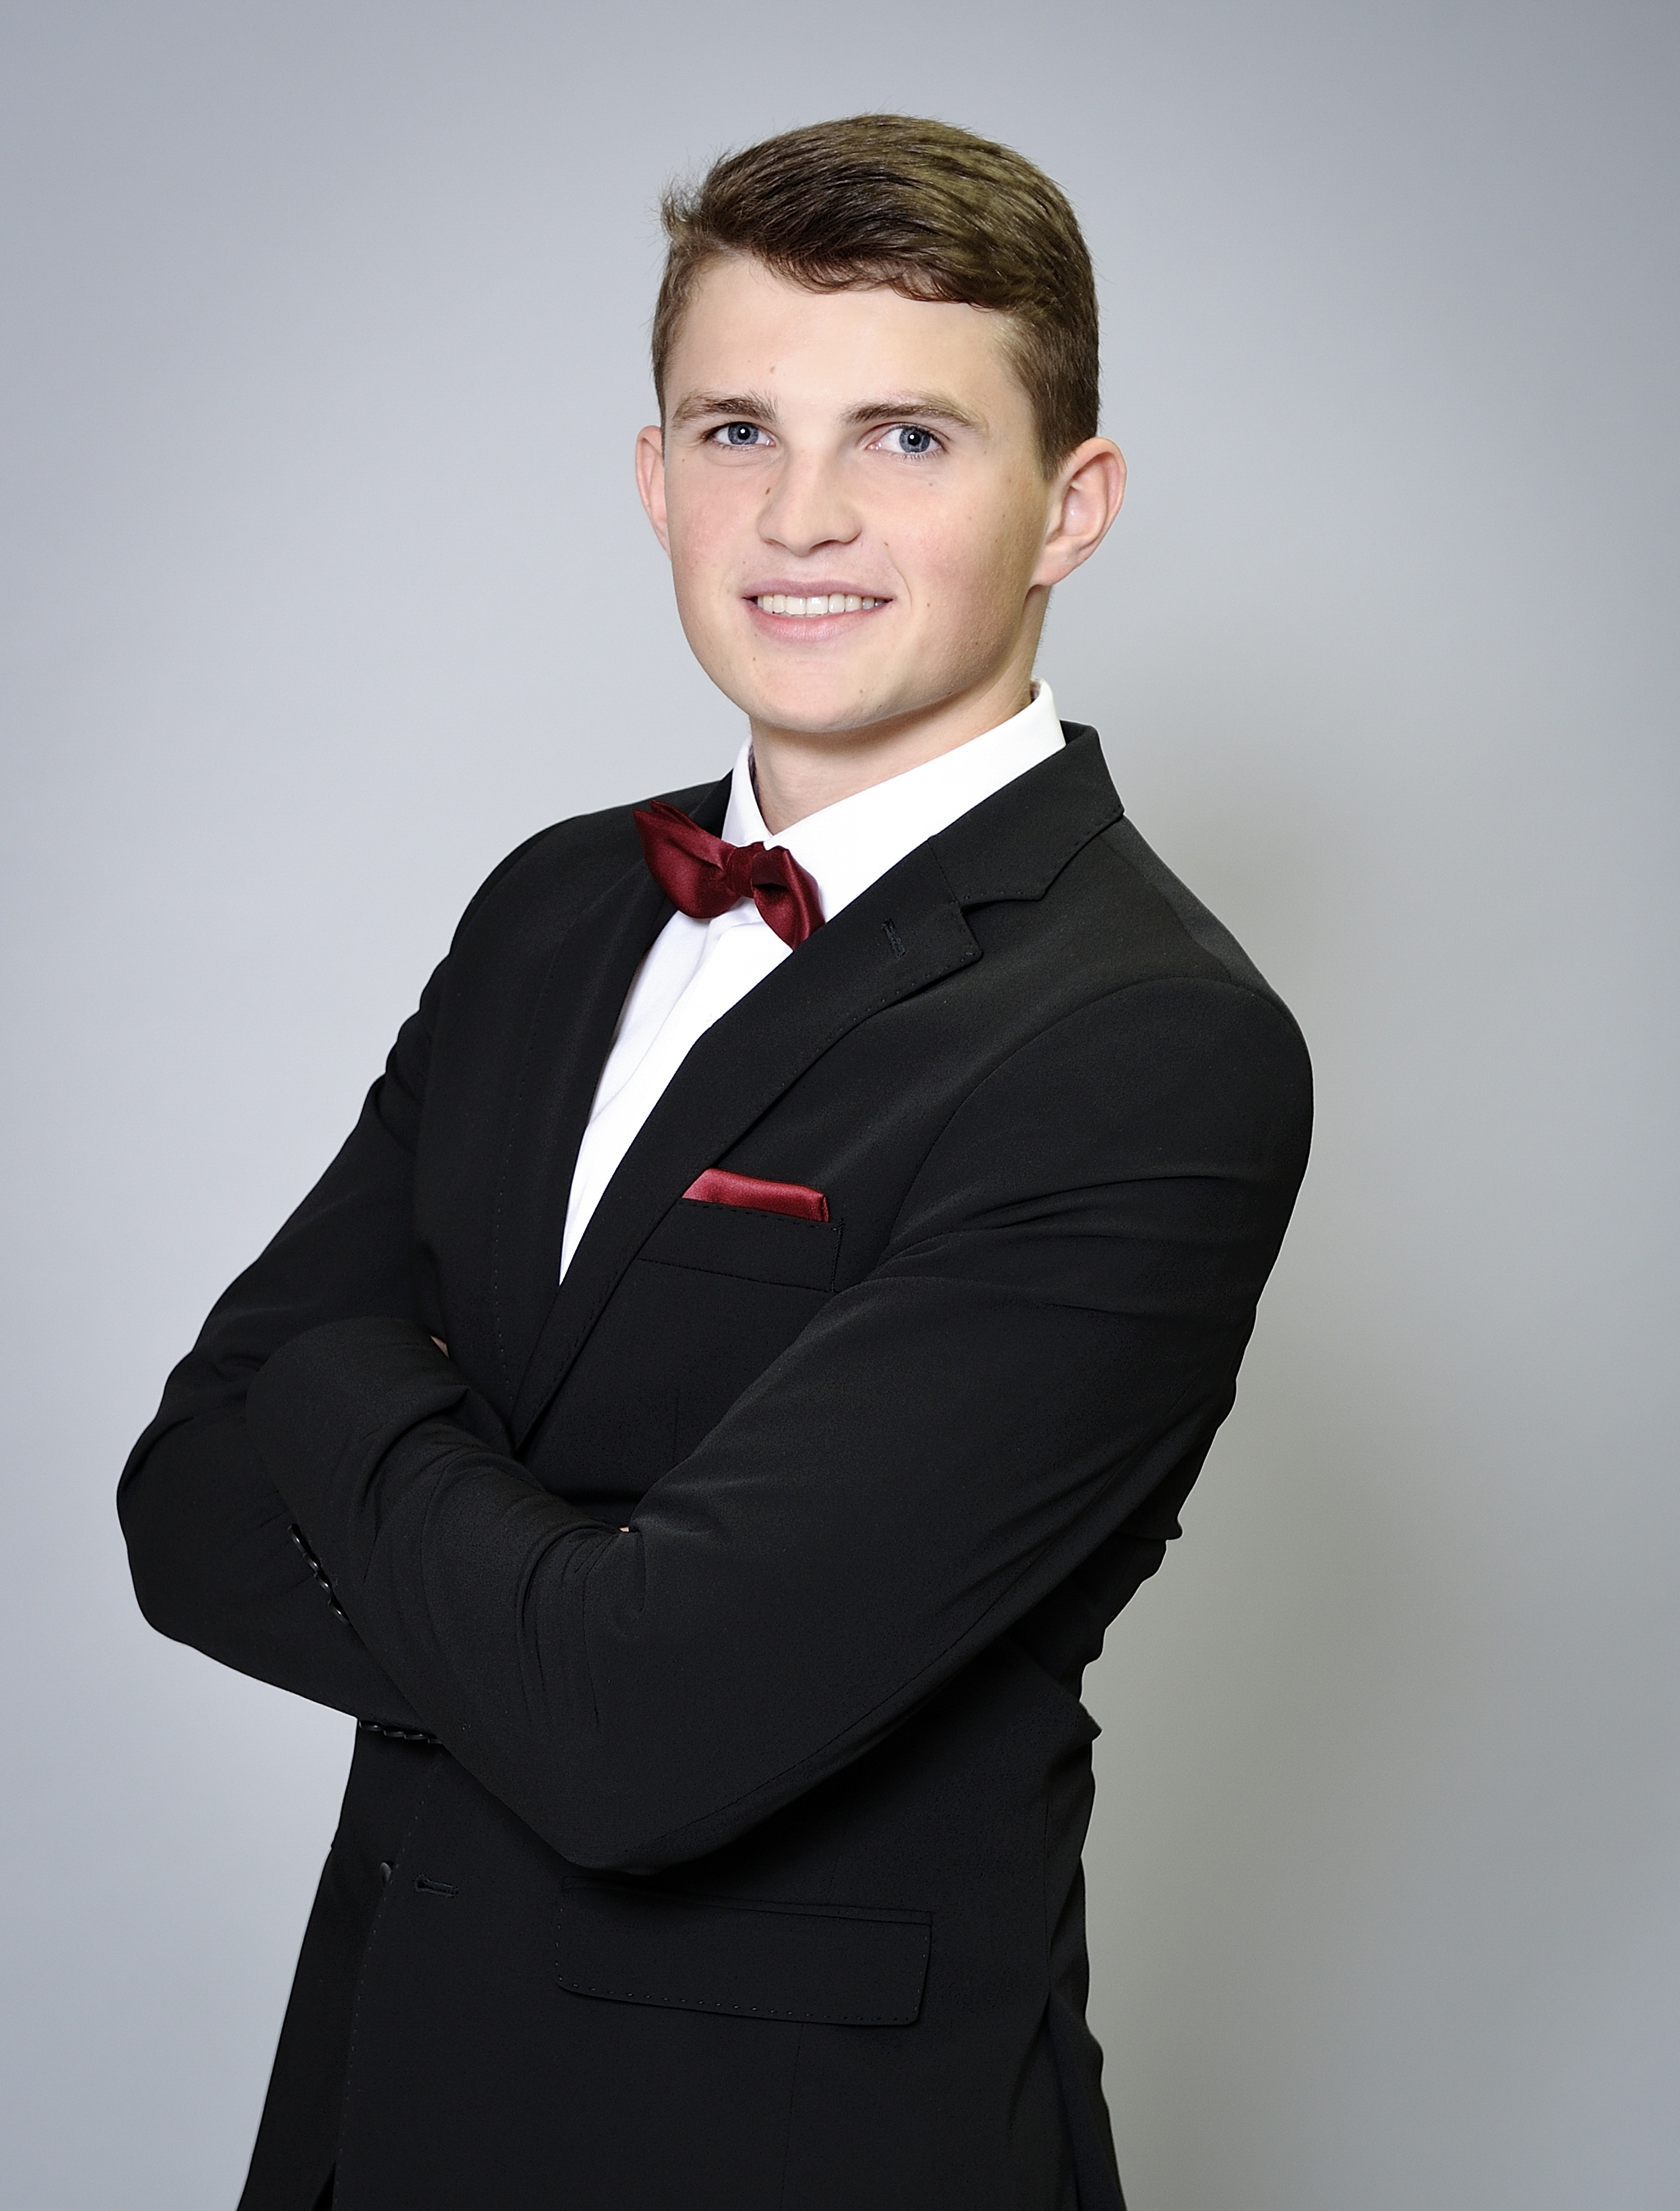
\includegraphics[width=0.3\textwidth]{fig/V.jpg}
\end{center}
\end{wrapfigure}
\mbox{}\\
\mbox{}\\
\textbf{Aufgabenbereich}:\\
Informatik\\
\textbf{Betreuer}:\\
Dipl-Ing. Manfred Steiner
\mbox{}\\
\mbox{}\\
\mbox{}\\
\mbox{}\\
\mbox{}\\
\mbox{}\\